\section{Projeto da arquitetura}
A arquitetura proposta neste trabalho é baseada em camadas e utiliza os estilos arquiteturais \textit{Client-Server} e \textit{Event-Based}. O modelo em camadas possibilita manter a organização, a separação de conceitos e responsabilidades dos recursos da arquitetura, viabilizando a integração e a comunicação entre os componentes através de conectores que podem ser definidos dinamicamente. No modelo em camadas, a conexão entre os componentes pode ser realizado tanto por eventos como por objetos compartilhados ou, através de leitura e escrita em um arquivo ou em uma base de dados. Porém, nesta arquitetura, foi utilizado somente eventos para comunicação entre os componentes. A escolha de eventos como principal conector entre os objetos foi feita principalmente por proporcionar comunicação assíncrona entre emissor e ouvinte e pelo fato de não acoplar os componentes, garantindo maior independência entre os objetos. Outro motivo da escolha de eventos, é o fato do Qt provê nativamente um mecanismo de comunicação através de eventos.\par


\subsection{Tecnologias utilizadas}
As tecnologias utilizadas consiste de todos os recursos que foram necessários para o desenvolvimento deste trabalho. O Qt e o \textit{QtCreator} foram os artefatos mais importantes, pois, forneceram os recursos e ferramentas para a construção das principais características da arquitetura. Dentre os recursos providos pelo Qt destaca-se os eventos, que permitem interligar objetos através de sinais e slots\footnote{funções javascript ou métodos de uma classe c++ invocados quando o sinal o qual estão conectados for emitido, recebendo em seus parâmetros os argumentos enviado pelo sinal.} ou \textit{signal handles}, e as APIs providas em classes C++ que integram os recursos da arquitetura, tais como, persistência de dados (via \textit{QSettings} e \textit{QSqlDatabase}) e rede (via \textit{QNetworkAccessManager}). O \textit{QtCreator} é uma IDE que possui recursos integrados à um projeto Qt e dentre os recursos destaca-se, facilidade de \textit{build} do projeto, construção do executável do aplicativo e o \textit{deploy} em um \textit{smartphone}. O \textit{QtCreator} também foi utilizado como editor de código fonte.


\subsection{Processos de desenvolvimento}
Esta arquitetura foi desenvolvida sob uma metodologia ágil com destaque para uma programação extrema e teste contínuo. A arquitetura recebeu alterações durante 10 meses e a primeira etapa de desenvolvimento introduziu o suporte aos plugins. O primeiro desafio foi desacoplar os plugins do arquivo QRC\footnote{QRC - Qt Resource Collection é um arquivo XML que mapeia os arquivos que serão empacotados no aplicativo.} e permitir que a aplicação carregasse-os dinamicamente. Também nesta primeira etapa, foi implementado alguns recursos associados aos plugins, como controle de cache dos arquivos QML, ordenação e \textit{parsing} das páginas (definido pelos plugins), além da criação de um componente genérico a ser extendido por todas as páginas do aplicativo. O controle de cache consiste em regenerar o cache dos arquivos QML após uma atualização para garantir o carregamento de mudanças em cada arquivo a cada release. O componente genérico foi definido como \textit{BasePage.qml} e será detalhado posteriormente, ele foi criado para garantir o atendimento de alguns requisitos mínimos de aparência, estrutura e simplificar a criação de páginas.\par

Na segunda etapa, foi implementado classes c++ para gerenciar as configurações da aplicação, classe utilitária com métodos a serem invocados pelos plugins para operações de baixo nível ainda não suportados pelo QML, além de classes para recursos extra providos pela arquitetura como diálogo para seleção de arquivo no android e IOS e envio de notificação para a bandeija do sistema.\par

Na terceira etapa, foi definido os layouts visuais suportados pela arquitetura e dois modelos foram implementados: O layout em pilha, que faz uso do container \textit{StackView} e o layout em linha, que faz uso do container \textit{SwipeView}, ambos do \textit{QuickControls}\footnote{Módulo do Qt que provê um conjunto de componentes para construção de interfaces gráficas utilizando QML.}. O suporte ao layout deve ser definido no arquivo de configuração principal (à ser detalhado posteriormente) \textit{config.json} e está presente no diretório raíz da arquitetura. Em etapas seguintes foi desenvolvido componentes visuais reutilizáveis, além das APIs para requisição HTTP e persistência de dados via \textit{QSLITE}. As imagens a seguir apresentam os layouts em pilha e em linha.

\begin{figure}[H]
	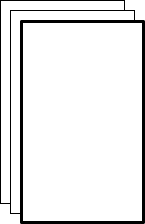
\includegraphics[scale=0.5]{stackview_wireframe}
	\centering
	\caption{Estrutura de um layout em pilha}
\end{figure}

No layout em pilha, o componente \textit{ToolBar.qml} será instanciado e posicionado no topo da janela do aplicativo. O \textit{ToolBar} fará um \textit{bind} com a página atualmente ativa, ou seja, a página que o usuário estiver visualizando. É importante destacar que em ambos os layouts, somente uma página pode ser visualizada por vez.

\begin{figure}[H]
	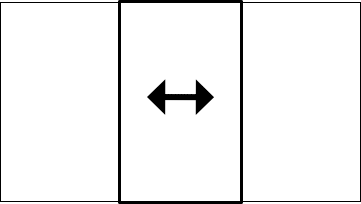
\includegraphics[scale=0.5]{swipeview_wireframe}
	\centering
	\caption{Estrutura de um layout em linha}
\end{figure}

No layout em linha, o componente \textit{TabBar.qml} será instanciado e posicionado no rodapé da janela do aplicativo e trabalhará em conjunto com o \textit{SwipeView}. A arquitetura suporta intercalar os dois layouts ao mesmo tempo, e um objeto \textit{Binding} do QML manterá o \textit{SwipeView} visível somente se não houver páginas na pilha do \textit{StackView}. No entanto o \textit{SwipeView} será instanciado somente se a propriedade \textit{usesSwipeView} for definida para \textit{true} no arquivo de configuração.\par


% ver link: https://pt.slideshare.net/adrianotavares/modelagem-arquitetural-e-viso-41-presentation %
\subsection{Visão Geral da Arquitetura}
A visão a seguir, apresenta um diagrama de pacotes e arquivos destacando uma visão lógica dos principais elementos da arquitetura e logo a seguir, é descrito o papel e o conteúdo de cada um deles.

\begin{figure}[H]
	\includegraphics[scale=0.5]{diagrama_geral_da_arquitetura}
	\centering
	\caption{Pacotes principais da arquitetura}
\end{figure}

\begin{description}
	\item[1] \textit{tcc.pro}: Arquivo de configuração de todo projeto Qt. Nele é definido os módulos do Qt a serem utilizados na aplicação, as classes c++ que serão compiladas e linkadas no executável, os aquivos qrc que mapeiam os componentes QML, as imagens e arquivos genéricos a serem empacotados no executável, além de módulos e arquivos de configuração para cada plataforma (linux, osx, android e ios). É neste arquivo que fica definido onde os plugins serão instalados no dispositivo.

	\item[2] \textit{main.cpp}: Arquivo que inicializa a aplicação. Esse arquivo é responsável por instanciar as classes do Qt que exibem a janela do aplicativo e o interpretador de código QML, além de classes da camada de aplicação, configuração e utilitários. O \textit{main.cpp} também é responsável por carregar os arquivos de tradução e registrar objetos no contexto da aplicação a serem utilizados pelos plugins.

	\item[3] \textit{config.json}: Arquivo de configuração principal desta arquitetura, pois define propriedades que indicarão alguns comportamentos iniciais e esolha de tipos de objetos a serem instanciados, tais como exibir os termos de uso na primeira inicialização do aplicativo (carregará o arquivo definido em \textit{assets/eula.html} definido pelo usuário da arquitetura), se tem login ou não (caso sim, instanciará um objeto que gerencia o perfil do usuário e a página de login), se usará layout em linha e etc. Os detalhes deste arquivo será apresentado em um tópico mais adiante.

	\item[4] \textit{src}: Diretório de código fonte. É onde está as classes c++ e componentes QML utilizados internamente e dispostos para plugins como componentes reusáveis. Esse diretório é sub-dividido em outros 5 diretórios que organizam as classes c++ por tipo de API a qual são resposáveis, e são eles: \textbf{core} -- contém classes do núcleo da aplicação dentre elas \textit{App}, \textit{PluginManager}, \textit{Notification} e \textit{Utils}; \textbf{database} -- contém classes da API de persistência de dados da aplicação; \textbf{extras} -- contém classes de customização de estilo no android; \textbf{network} que mantém as classes da API de rede da aplicação e \textbf{qml} que contém os arquivos qml sub-divididos em \textit{private} e \textit{public}, sendo os componentes "privado" os que são utilizados internamente pela aplicação e os componentens públicos os que são reutilizados pelos plugins.

	\item[5] \textit{plugins}: Diretório de plugins. Cada plugin deve obrigatóriamente estar em um sub-diretório com no mínimo um arquivo de configuração de nome \textit{config.json} e os arquivos QML necessirários para o seu funcionamento. Os detalhes das propriedades requeridas para o carregamento de um plugin serão descritas em um tópico posterior.

	\item[6] \textit{translations}: Diretório contendo os arquivos de tradução. Os arquivos de tradução devem ser gerados ou atualizados antes de cada release do aplicativo. Um arquivo de resources \textit{translations.qrc} existe neste diretório e deve ser utilizado para mapear os arquivos de idioma suportados pelo aplicativo. Cada arquivo de tradução deve ser nomeado seguindo o padrão \textit{language\_COUNTRY} com extensão \textit{ts}, por exemplo: \textit{pt\_BR.ts}. Ao iniciar a aplicação, no arquivo \textit{main.cpp}, será identificado o \textit{locale} que define o idioma utilizado no dispositivo e o arquivo correspondente será carregado para que os textos visíveis sejam traduzidos para o usuário. Para gerar as traduções, deve-se utilizar o comando \textit{lupdate *.pro} (na raíz do projeto) para criar ou atualizar o arquivo \textit{ts} principal.

	\item[7] \textit{android}: Diretório contendo os arquivos de configuração do aplicativo para a plataforma android. Outros sub-diretórios guardam arquivos do \textit{gradle} utilizados para o \textit{build} do APK, ícones do lançador do aplicativo e classes java, além de uma versão da lib \textit{openssl} compilada para o funcionamento de requisições HTTP.

	\item[8] \textit{assets}: Diretório contendo imagens e arquivos de configuração do \textit{qtquickcontrols2} além de um arquivo html que pode ser usado para exibir os termos de uso do aplicativo quando utilizado necessário (a propriedade \textit{showEula} seja definido para true no \textit{config.json}). Um arquivo de \textit{resources} \textit{assets.qrc} mapeia todos os arquivos contidos neste diretório e pode ser usado para adicionar outros arquivos a serem empacotados no aplicativo.

	\item[9] \textit{ios}: Diretório contendo os arquivos de configuração do aplicativo para a plataforma ios. Pode conter os ícones do aplicativo, além de imagens diversas requeridas pela plataforma tais como as imagens de \textit{splash-screen}, além do arquivo de configuração \textit{Info.plist} que define nome, versão e recursos do sistema requerido pelo aplicativo.
\end{description}


\subsection{Arquitetura de plugins}
As funcionalidades de um aplicativo baseado nesta arquitetura devem ser implementadas através de plugins, atendendo aos requisitos levantados para o aplicativo a ser desenvolvido utilizando apenas qml. Os plugins são independentes entre sí e podem incluir arquivos qml, txt, html e imagens em seu diretório. Qualquer componente de um plugin pode reutilizar os componentes públicos usando a diretiva \textit{import "qrc:/src/qml/"}. Os plugins estão desacoplados do núcleo da aplicação e serão conhecidos em tempo de execução. Ao adicionar um novo plugin no diretório \textit{plugins}, ele será carregado no próximo \textit{build} do projeto. Para que um plugin seja identificado pelo objeto gerenciador de plugins para ser carregado na aplicação, é necessário obedecer a três restrições: 1º) estar em um sub-diretório dentro de \textit{plugins}; 2º) conter um arquivo \textit{config.json} e, 3º) conter pelo menos um arquivo qml visual ou \textit{listener}. Os \textit{listeners} são componentes não visuais que observam eventos da aplicação. O arquivo \textit{config.json} de um plugin deve ser um objeto contendo as seguintes propriedades:  
\begin{enumerate}
	\item \textit{name} (string): o nome do plugin. Deve ser preenchido para que o plugin seja identificado pelo objeto gerenciador de plugins;

	\item \textit{description} (string): um texto que descreve o plugin. Deve ser definido, caso contrário o plugin não será adicionado a lista de plugins da aplicação;

	\item \textit{pages} (array): uma lista de objetos que indentifica as páginas do plugin que serão acessadas a partir do menu ativo no aplicativo e deve ser preenchido se a propriedade \textit{listeners} estiver vazia;

	\item \textit{listeners} (array): uma lista de strings que indentifica os arquivos do plugin (componentes qml não visuais) que serão instanciados como observadores de eventos. O preenchimento dessa propriedade é opcional e pode ser preenchida mesmo que a propriedade \textit{pages} seja preechida.
\end{enumerate}

Cada objeto em \textit{pages} poderá conter as seguintes propriedades que serão lidas pelos componentes que definem os menus durante a inicialização do aplicativo:

\begin{itemize}
	\item \textit{qml} (string): O nome do arquivo correspondente a página. Se essa propriedade não for definida, a página não será carregada.

	\item \textit{title} (string): O título correspondente a página a ser exibido no menu. Esse valor também é requerido, se não for definido, a página não será carregada.

	\item \textit{icon} (string) (opcional): O nome de um ícone do \textit{Awesome Icons} que será exibido no menu, em conjunto com o título. Se esse valor não for definido, um ícone padrão será utilizado.

	\item \textit{roles} (array): Uma lista de strings contendo os nomes de perfil de usuário que poderão acessar a página. Esse array será útil somente se a aplicação definir o tipo de perfil do usuário no objeto \textit{UserProfile.profile}. Esse valor é opcional, caso não for definido, será setado um array vazio. Porém, se for definido o perfil do usuário no objeto \textit{profile} e essa string não tiver nesta propriedade (\textit{roles}), a página não será exibida.

	\item \textit{order} (integer): Um valor numérico que define a ordem em que a página será exibida na lista de itens nos menus. O desenvolvedor deverá definir um valor acima de zero e quanto maior o valor, maior a prioridade na lista de itens.

	\item \textit{isLoginPage} (boolean): Um valor boleano que indica se a página representa a tela de login do aplicativo e deve ser definido se o valor da propriedade \textit{usesLogin} for definido para true no \textit{config.json} do projeto. Se o aplicativo usa login, o \textit{path} da página definida como login será persistido pois será lido por funções internas do aplicativo na inicialização e quando o usuário fizer \textit{logout}. Se mais de uma página for definida como \textit{loginPage} entre os plugins, será utilizada a última página identificada pelo gerenciador de plugins.

	\item \textit{isHomePage} (boolean): Um valor boleano que indica se a página corresponde a primeira página exibida para o usuário. Se for definido para \textit{true}, o \textit{path} desta página será persisitido e será carregada após o login. No entanto, se o aplicativo não usa login, o aplicativo carregará a página definida como \textit{homePage} na inicialização e será a primeira página exibida para o usuário. Essa propriedade é requerida no modo de layout em pilha e deve ser definida somente pela página correspondente. Se mais de uma página for definida como \textit{homePage}, será utilizada a última página identificada pelo gerenciador de plugins.

	\item \textit{showInDrawer} (boolean): Um valor boleano que indica se a página poderá ser exibida no menu de layout em pilha. O menu de layout em pilha será instanciado por padrão no layout em pilha, porém, também pode ser instanciado no layout em linha, basta definir a propriedade \textit{usesDrawer} para \textit{true} no arquivo de configuração. O layout em linha utiliza uma barra de botões como menu e com isso, é possível permitir acesso a páginas diferentes a partir dos dois menus.

	\item \textit{showInTabBar} (boolean): Um valor boleano que indica se a página poderá ser exibida no menu de layout em linha. O objetivo desse flag é permitir exibir páginas diferentes nos menus quando o \textit{Drawer} menu estiver sendo utilizado, permitindo assim, exibir páginas diferentes nos dois menus.
\end{itemize}

As páginas serão instanciadas sob demanda quando o aplicativo tiver utilizando o layout em pilha, neste caso quando o usuário clicar em um item da lista no menu, a página correspondente será instanciada e ficará visível para o usuário. No layout em pilha, o menu é exibido pelo componente \textit{Menu.qml} que consiste de uma instância do objeto \textit{Drawer} do \textit{QuickControls} e as páginas serão listadas verticalmente. A figura a seguir apresenta um exemplo deste menu com uma lista simples de páginas.

\begin{figure}[H]
	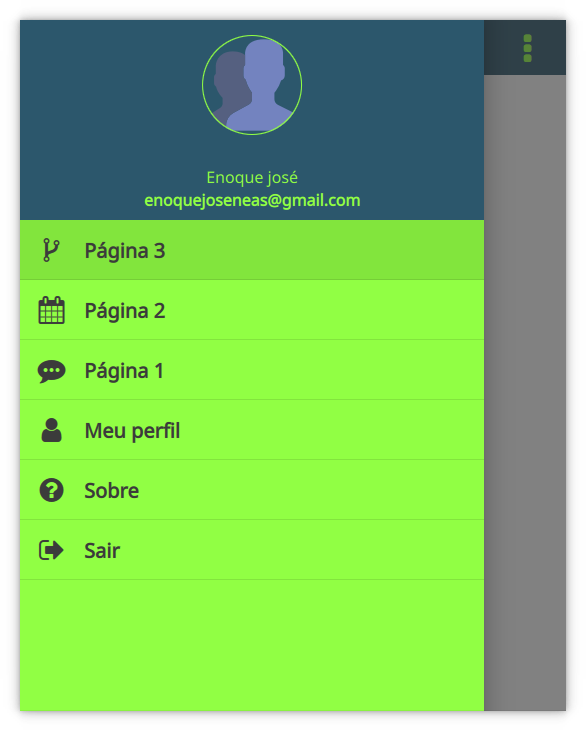
\includegraphics[scale=0.5]{exemplo_menu_layout_em_pilha}
	\centering
	\caption{Lista de páginas exibidas no menu de layout em pilha}
\end{figure}

Quando o layout em linha estiver sendo utilizado, uma lista horizontal de botões será acidionado no rodapé da janela do aplicativo permitindo ao usuário alternar entre as páginas disponíveis. Porém, no layout em linha, todas as páginas serão instanciadas no início da aplicação e terá um botão associado a cada página. No layout em linha, o menu corresponde ao componente \textit{TabBar.qml} também do \textit{QuickControls} com algumas modificações. A figura a seguir apresenta um exemplo deste menu com uma lista simples de páginas. A exibição do título da página pode ser ocultada setando a opção \textit{showTabButtonText} para false no arquivo de configuração do projeto.

\begin{figure}[H]
	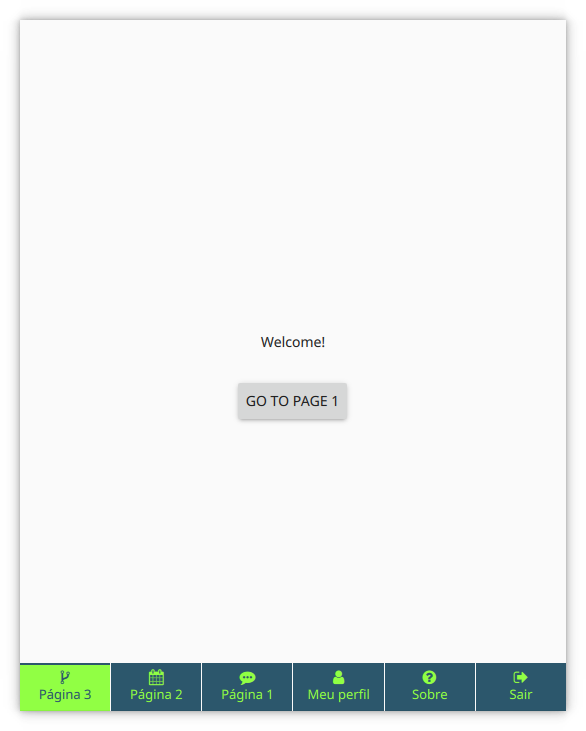
\includegraphics[scale=0.5]{exemplo_menu_layout_em_linha}
	\centering
	\caption{Lista de páginas exibidas no menu de layout em linha}
\end{figure}


\subsubsection{Gerenciamento de plugins}\label{sec:solucao-desenvolvida}
A classe \textit{PluginManager} é responsável por carregar os plugins, percorrendo todos os arquivos dentro do diretório \textit{plugins} e analizando as propriedades definida no arquivo \textit{config.json} de cada plugin. Em cada arquivo, é verificado as propriedades definida para cada página adicionando-a como objeto em um array. Após ler todos os plugins, o array de objetos é persistido nas configurações da aplicação para que na próxima inicialização não precise iterar novamente o diretório, lendo as definições dos plugins das configurações, exceto se houver uma atualização da aplicação ou quando a aplicação é executada em modo \textit{debug}. A cada inicialização, é feito uma verificação da versão do aplicativo, que também é persistida nas configurações, se houver diferença entre versão em execução da versão salva na execução anterior (se existir), os plugins serão recarregados. Além disso, esta classe também é reponsável por deletar todos os arquivos de cache contido no diretório de cache da aplicação a cada release. Outra responsabilidade dessa classe, é a criação da tabela de banco de dados do plugin se o plugin dispor de um arquivo \textit{plugin\_table.sql} em seu diretório. O banco de dados da aplicação é criado por um objeto que gerencia as operações de persistência e será detalhado em outro tópico. O diagrama a seguir, apresenta as operações e atributos da classe \textit{PluginManager}.

\begin{figure}[h]
	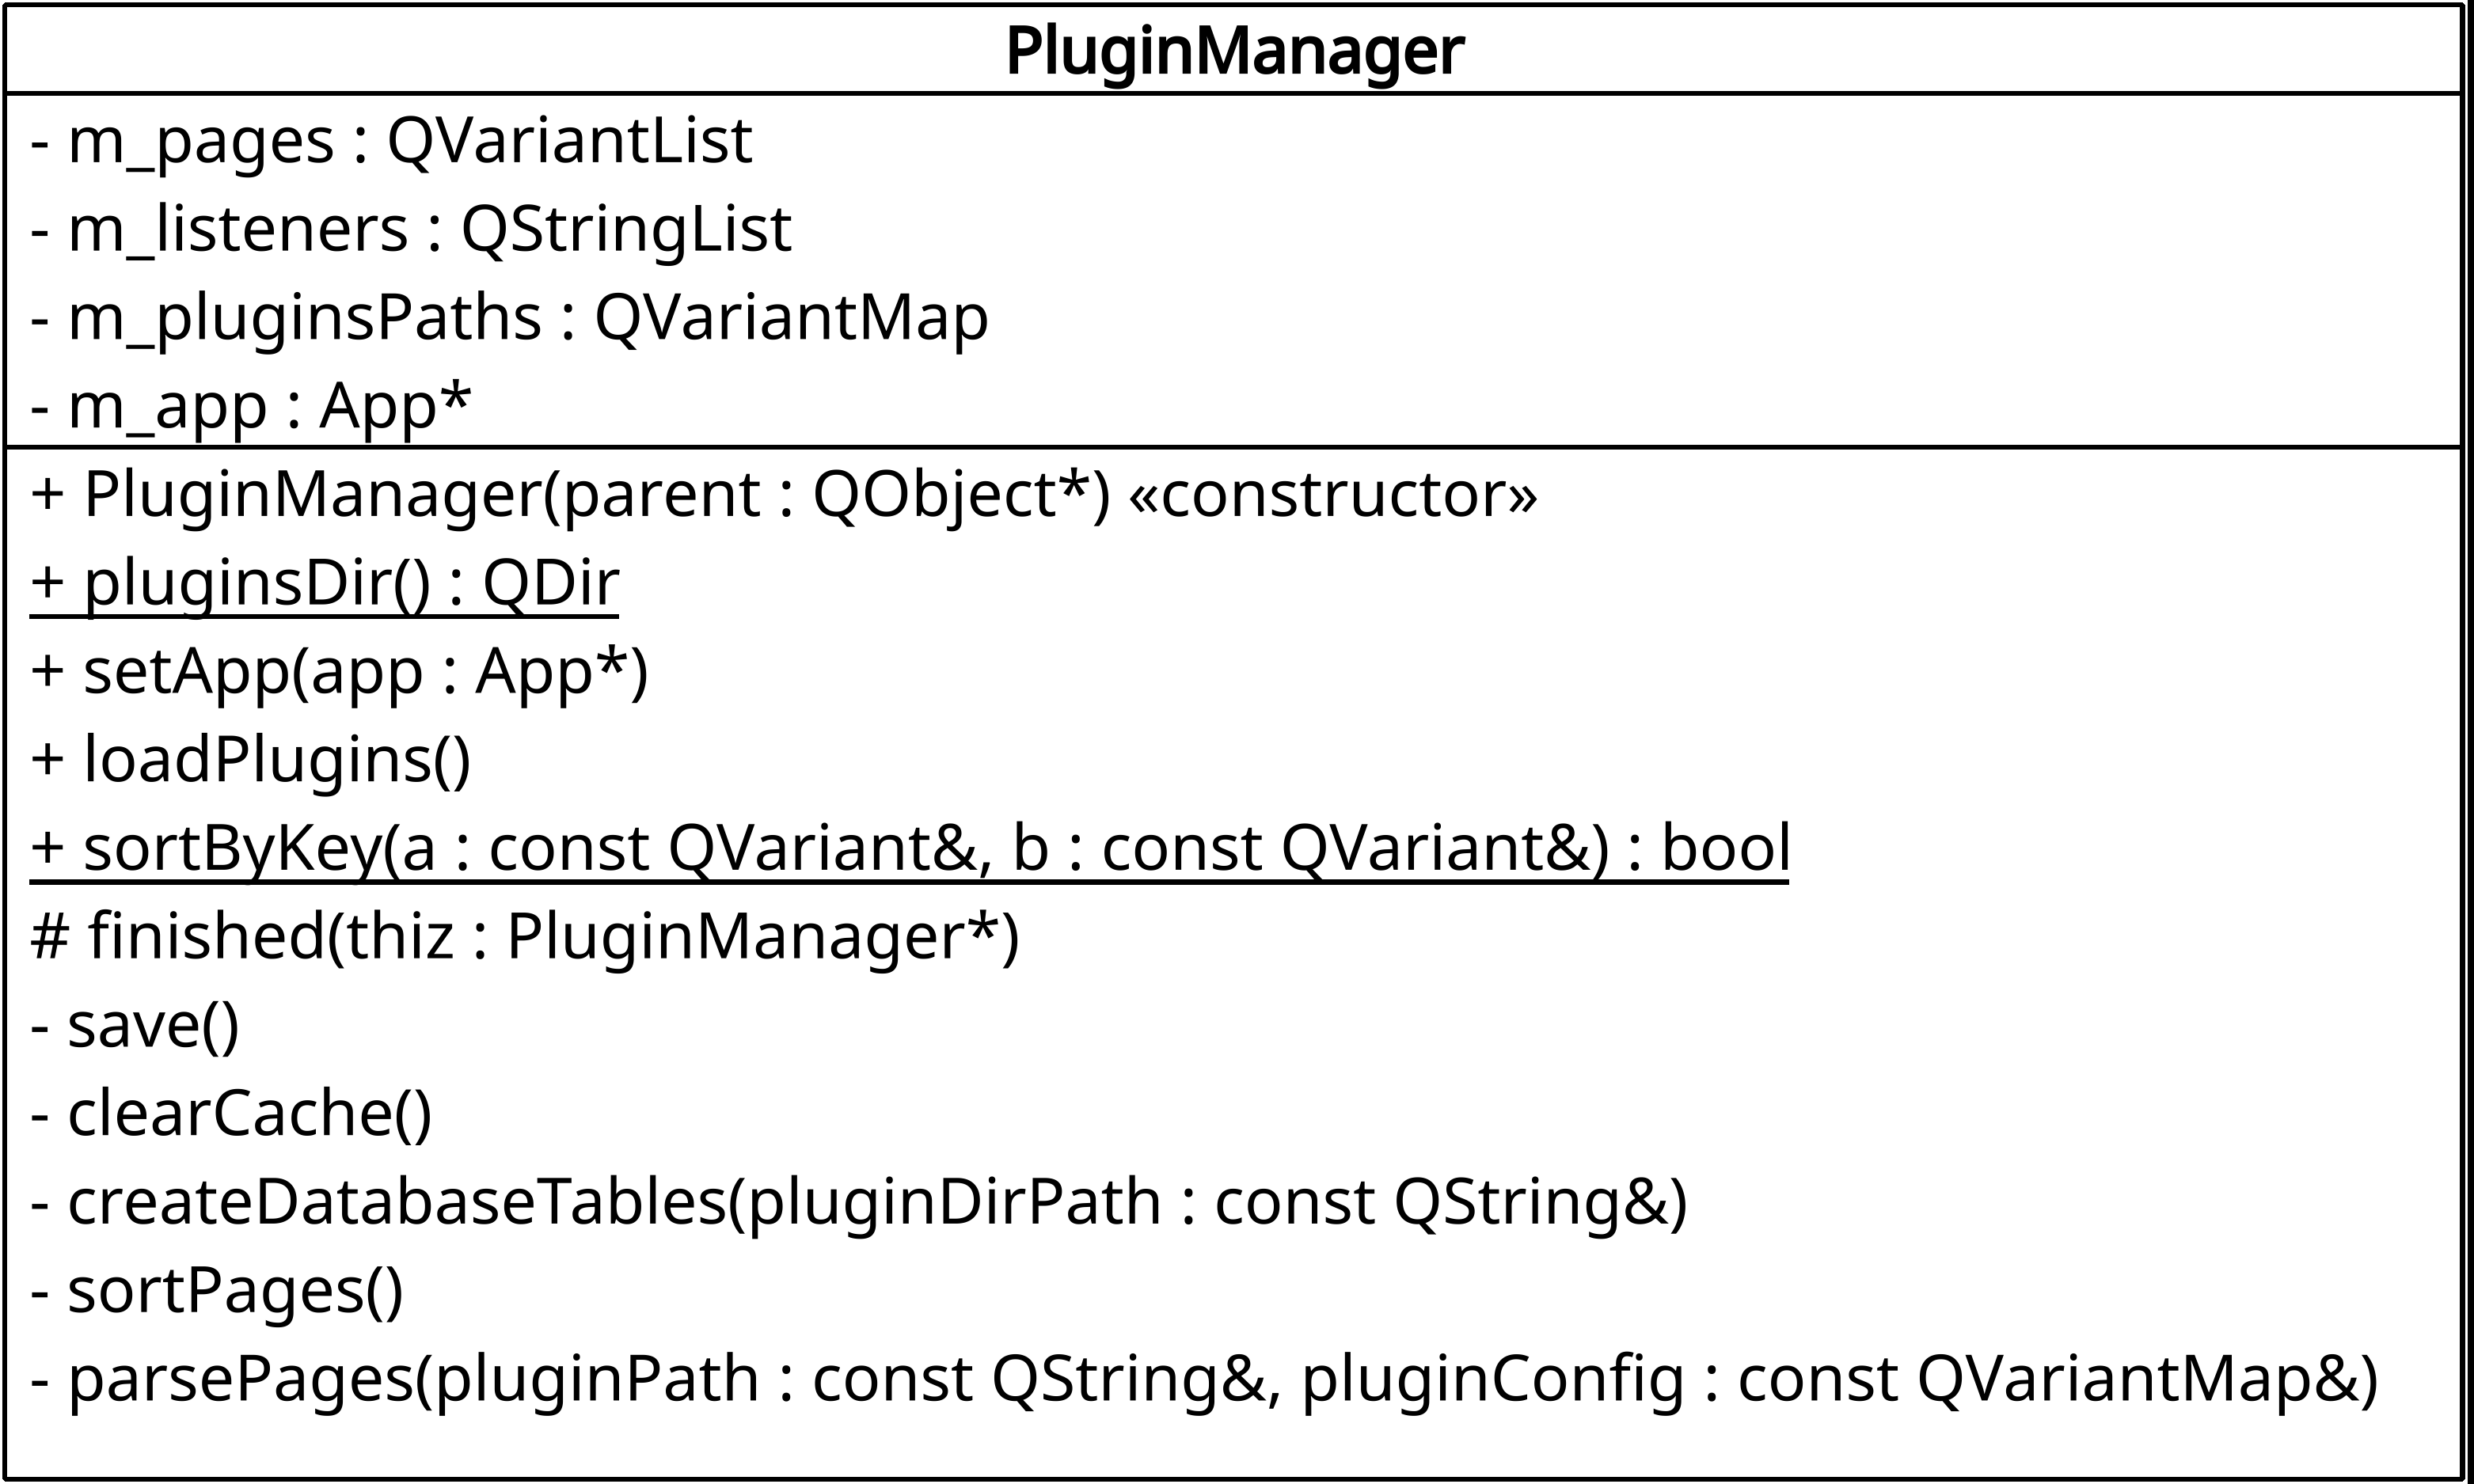
\includegraphics[width=8cm]{diagrama_de_classe_PluginManager}
	\centering
	\caption{Diagrama da classe PluginManager}
\end{figure}

A instância de \textit{PluginManager} é criada pelo objeto \textit{app} na inicialização do aplicativo e o processo de carregamento dos plugins é feito antes de instanciar qualquer componente visual, na invocação do método \textit{loadPlugins}. O objeto \textit{pluginManager} será destruido após o carregamento dos plugins para manter baixo consumo de memória pelo aplicativo.


\subsection{A classe App}\label{sec:solucao-desenvolvida}
A classe \textit{App} é um componente importante nesta arquitetura, suas responsabilidades consiste de instanciar \textit{PluginManager} que carregará os plugins, carregar o arquivo \textit{config.json} principal que contém os parâmetros da aplicação e gerenciar a persistência das configurações da aplicação via \textit{QSettings}\footnote{Uma classe do Qt que fornece um mecanismo de leitura e escrita de dados no dispositivo através de métodos parametrizados.}. A classe \textit{App} é instanciada na inicialização do aplicativo e é registrada no contexto da aplicação para que os plugins e componentes qml possam invocar seus métodos públicos definidos como \textit{Q\_INVOKABLE}, como por exemplo, o método \textit{readSettings} que retorna um tipo genérico de dado, lido das configurações do aplicativo através de algum parâmetro que identifique o dado a ser lido. Outra tarefa que corresponde a esta classe, é a criação de uma conexão com a atividade do aplicativo no android, que corresponde a uma classe. Essa atividade poderá receber parâmetros de eventos como \textit{push notification} ou token de registro no \textit{Firebase}, quando utilizado pela aplicação. O processo de registro do token e o recebimento de notificações via push é feito por objetos java em um processo separado da aplicação, e quando a aplicação estiver em execução, a atividade do aplicativo passará os argumentos recebidos do push ou token para a aplicação através de uma chamada ao método estático \textit{fireEventNotify} da classe \textit{App}.\par

No iOS, o objeto correspondente a APP também poderá receber argumentos vindos do \textit{QtAppDelegate} objeto que carrega os requisitos da plataforma e inicializa a aplicação. Os argumentos que podem ser recebidos são o \textit{token} de registro no \textit{Firebase} e mensagens de notificações via push.

\begin{figure}[h]
	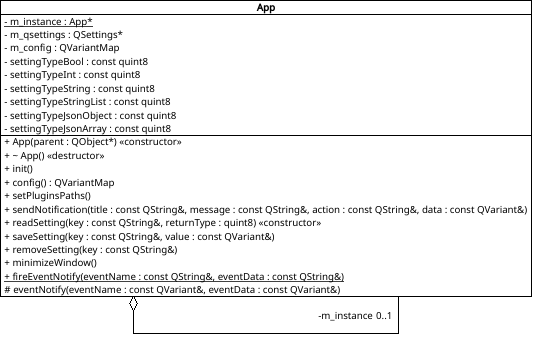
\includegraphics[scale=0.6]{diagrama_de_classe_App}
	\centering
	\caption{Diagrama da classe App}
\end{figure}

A classe \textit{App} também é responsável por definir o estilo de widgets utilizado pelos componentes qml. O tipo de estilo deve ser definido pelo usuário no arquivo de configuração \textit{config.json}, na propriedade \textit{applicationStyle} e será passado diretamente para o objeto \textit{QQuickStyle}. Os possíveis valores para esta propriedade serão detalhados na sessão que descreve o arquivo \textit{config.json}. A instãncia desta classe adicionará no objeto \textit{Config} a cada inicialização, uma propriedade contendo o path de cada plugin para que os plugins possam acessar os arquivos em seu diretório usando essa propriedade. Exemplo: Considerando que \textit{Session} seria um plugin, os arquivos deste plugin poderiam acessar outros arquivos fazendo uma referência do tipo \textit{Config.plugins.session + "File2.qml"}.


\subsection{O arquivo config.json}\label{sec:solucao-desenvolvida}
O arquivo \textit{config.json} é um elemento importante desta arquitetura, ele é utilizado como arquivo de configuração geral do aplicativo, porém, suas informações não serão persistidas. O conteúdo deste arquivo será repassado para a aplicação como um objeto javascript e o usuário poderá adicionar propriedades a serem lidas pelos plugins. No entanto, as propriedades fornecidas no modelo desta arquitetura não devem ser removidas, pois, componentes internos fazem uso das propriedades definidas neste arquivo. Os plugins poderão ler essa propriedade acessando \textit{Config.\_nome\_da\_propriedade}. As principais propriedades e seus possíveis valores podem ser entendidas a seguir:

\begin{itemize}
	\item \textit{appName} (string): O nome do aplicativo. Este valor será setado em \textit{QApplication.setApplicationName} na inicialização do aplicativo;

	\item \textit{appDescription} (string): Uma descrição sobre o aplicativo. Essa propriedade é opcional;

	\item \textit{organizationName} (string): O nome da organização. Este valor será setado em \textit{QApplication.setOrganizationName} na inicialização do aplicativo e é será utilizado internamente pelo Qt para definir o nome do diretório de configurações da aplicação;

	\item \textit{organizationDomain} (string): O domínio da organização, como por exemplo \textit{qt.project.org}. É utilizado pelo Qt internamente.

	\item \textit{applicationStyle} (string): O nome do estilo a ser aplicado nos widgets (\textit{Button}, \textit{TabBar}, \textit{ToolTip} e etc.). Os possíveis valores são: \textit{Material}, \textit{Universal} e \textit{Default}. O valor dessa propriedade será passada pelo objeto \textit{App} para \textit{QQuickStyle.setStyle};

	\item \textit{forceEulaAgreement} (boolean): Um valor boleano que inidica se a aplicação deverá exigir do usuário confirmação de aceitação dos termos de uso para continuar usando o aplicativo. Esse valor só terá efeito se a propriedade \textit{showEula} for definida para \textit{true};

	\item \textit{hasLogin} (boolean): Um valor boleano que indica se o aplicativo deverá carregar uma página de login na inicialização. Se definido para \textit{true}, a aplicação irá utilizar a página (dentre os plugins) que definiu \textit{isLoginPage} para \textit{true}, identificada pelo gerenciador de plugins durante o carregamento dos plugins;

	\item \textit{showEula} (boolean): Um valor boleano que inidica se a aplicação exibirá para o usuário uma página contendo os termos de uso do aplicativo. Caso seja setado para \textit{true}, o arquivo \textit{assets/eula.html} será carregado e exibido na página incial, na inicialização do aplicativo. Após o usuário ler e acitar os termos de uso, o usuário irá para a página de login ou \textit{home page} se tiver sido definida;

	\item \textit{showTabButtonText} (boolean): Um valor boleano que indica se o título da página será exibida no botão do menu em linha, que consite de um objeto \textit{TabButton} do \textit{QuickControls}. Essa propriedade só terá efeito quando a aplicação tiver usando o layout em linha.

	\item \textit{usesSwipeView} (boolean): Um valor boleano que indica se o layout principal do aplicativo será em linha, que consiste na utilização de um container do \textit{QuickControls} \textit{SwipeView}. No entanto, o container responsável pelo layout em pilha, \textit{StackView} ainda continuará disponível na aplicação, porém como container secundário. Um objeto fará o \textit{Binding} entre ambos os containers, ocultando o \textit{SwipeView} quando alguma página for adicionada a pilha do \textit{StackView}. No \textit{SwipeView} o usuário poderá alternar entre as páginas deslizando horizontalmente.

	\item \textit{usesDrawer} (boolean): Um valor boleano que indica se o menu lateral usado no layout em pilha, será instanciado. Esse componente corresponde a um objeto \textit{Drawer} do \textit{QuickControls}. No entando, esse flag terá efeito apenas no layout em linha, ou seja, se \textit{usesSwipeView} for true, pois no layout em pilha ele será instanciado mesmo que esse flag seja falso. O objetivo dessa propriedade é permitir que o programador possa utilizar o menu lateral quando o layout for me linha, intercalando as páginas que serão visíveis em cada um dos menus através das propriedades \textit{showInDrawer} e \textit{showInTabBar} na configuração de cada página no arquivo de configuração do plugin.

	\item \textit{showDrawerImage} (booleano): Um valor boleano que indica se a imagem do \textit{Drawer} menu será carregada. Por padrão a imagem não será exibida.

	\item \textit{restService} (objeto): Um objeto contendo as definições do serviço REST, como url base e o tipo de autenticação seguido dos respectivos parâmetros a serem enviados nas requisições HTTP como token ou usuário e senha. As propriedades para \textit{restService} são: 

	\begin{itemize}
		\item \textit{authentication} (objeto): Um objeto que define o tipo de autenticação e pode conter as propriedades \textit{basic authentication} ou \textit{headerToken}. Para o \textit{basic authentication}, deve ser informado o \textit{userName} e o \textit{password}. No \textit{headerToken}, deve ser informado o nome da chave em \textit{keyName} e a string contendo o \textit{hash}.

		\item \textit{baseUrl} (string): A url base do serviço REST. Essa propriedade será utilizada pelo objeto \textit{RequestHttp} nos métodos de requisição ao serviço REST GET, POST e etc. O objetivo é que nas páginas que fazem requisições HTTP adicionem apenas o \textit{path}, a fim de reduzir e simplificar o código. Com isso, uma alteração futura da url do serviço REST seria feita apenas no arquivo de configuração. Por exemplo, uma requisição do tipo GET pode ser feita da seguinte forma: \textit{requestHttp.get("/get-messages?page=2")}. Internamente, o objeto gerenciador de requisições concatenará essa propriedade com o path.

		\item \textit{baseImagesUrl} (string): A url base dos arquivos de imagens, caso o serviço REST utilize uma url diferente ou um sub-domínio para os resources.
	\end{itemize}

	\item \textit{fontSize} (objeto): Um objeto com as definições de valores inteiros para os tamanhos de fonte a serem utilizadas em elementos textuais como \textit{labels}. Essa propriedade possui 4 atributos: \textit{small}, \textit{normal}, \textit{large} e \textit{extraLarge};

	\item \textit{theme} (objeto): Um objeto com as definições de cores utilizada nos elementos visuais, tais como Botões, \textit{ToolBar}, \textit{TabBar}, cor de fundo das páginas e etc.;

	\item \textit{events}: (objeto): Um objeto que mapeia os identificadores de eventos, baseados em um par de strings \textit{nome-do-evento.valor}. Essa propriedade deverá ser utilizada por objetos e componentes internos para identificarem de qual evento estão sendo notificados, a fim de padronizar os nomes dos eventos e reduzir a replicação de strings na aplicação. O objeto \textit{App} adiciona treze nomes de eventos, alguns são utilizados somente por objetos internos, outros podem ser utilizados pelos plugins para executarem ações específicas em dado momento. Esses eventos serão descritos a seguir:
	\begin{itemize}
		\item \textit{cameraImageSaved} (string): Utilizado para notificar observadores que uma imagem foi capturada pela câmera do dispositivo e salva localmente. A url da imagem salva será passado no segundo argumento do evento;

		\item \textit{cancelSearch} (string): Utilizado pelo \textit{ToolBar} para indicar que o campo de busca não está ativo, para que a página corrente atualize o conteúdo para o usuário. O \textit{ToolBar} possui um campo texto para pesquisa e ficará visível quando a página alterar o valor da propriedade \textit{toolBarStatus} para \textit{"search"}. Essa funcionalidade permitirá que uma página filtre os resultados exibidos na sua \textit{view}, recebendo em um atributo string \textit{searchText} o valor digitado no campo. Esse recurso funcionará somente no layout em pilha. O usuário poderá cancelar a busca clicando em um botão voltar que ficará visível ao lado do campo de busca, nesse momento, o sinal \textit{"cancelSearch"} será disparado;

		\item \textit{logoutApplication} (string): Utilizado pelo objeto \textit{UserProfile} para atualizar o status da propriedade \textit{isUserLoggedIn} para false e em seguida, focar na página de login. Esse evento deve ser utilizado para evitar o acesso direto ao objeto \textit{UserProfile} pelos plugins, e deve ser emitido sempre que desejar remover todas as páginas da pilha (caso o layout seja em pilha) ou desabilitar o acesso as páginas do aplicativo (no layout em linha);

		\item \textit{newIntentPushMessage} (string): Esse evento é utilizado pelas APIs de notificação do android e iOS quando o usuário clicar em uma notificação na bandeija do sistema contendo algum dado na notificação. O segundo parâmetro do sinal \textit{eventData} conterá os dados da mensagem em uma string e caso seja um json, é necessário fazer o parse;

		\item \textit{newPushMessage} (string): Esse evento será disparado sempre que uma notificação via push chegar no dispositivo e o mesmo estiver em execução em \textit{foreground} ou \textit{background}. Ele é disparado a partir dos serviços de notificação que executam em outro processo e serão passados para a aplicação através de uma conexão entre o objeto java \textit{QtAtivity} no android e o \textit{QtAppDelegate} no iOS. O segundo parâmetro do sinal \textit{eventData}, conterá os dados da mensagem em uma string e caso seja um objeto json, é necessário fazer o parse;

		\item \textit{newPushNotificationToken} (string): Esse evento será emitido quando o token de registro no serviço do Firebase for realizado. Esse evento será disparado pelos objetos do \textit{Firebase}, que executam em outro processo e serão passados para a aplicação através de uma conexão entre o objeto java \textit{QtAtivity} no android e o \textit{QtAppDelegate} no iOS. O segundo parâmetro do sinal \textit{eventData} conterá os dados da mensagem em uma string e caso seja um objeto json, é necessário fazer o parse;

		\item \textit{openDrawer} (string): Esse sinal deve ser disparado para que o \textit{Drawer Menu} seja aberto, evitando uma chamada direta ao objeto. O \textit{ToolBar} por exemplo, emite esse sinal quando o usuário clicar no ícone do menu;

		\item \textit{popCurrentPage} (string): Esse evento deve ser disparado sempre que uma página precise ser removida da pilha do \textit{StackView} (container do layout em pilha). Inicialmente esse sinal é disparado pelo \textit{ToolBar} e ouvido pelo \textit{PageStack}.

		\item \textit{refreshDrawerPages} (string): Esse evento pode ser utilizado para atualizar a lista de itens no \textit{Drawer} menu permitindo adicionar páginas dinamicamente.

		\item \textit{requestUpdateUserProfile} (string): Esse evento deve ser emitido quando houver um perfil de usuário no aplicativo e permitirá atualizar as informações ou dados do usuário no objeto \textit{UserProfile.profile}. Por exemplo, uma página que permite editar os dados do usuário em um formulário, ao clicar em atualizar alguma informação, a página poderá emitir esse evento passando como argumento um objeto contendo as informações do usuário no estilo \textit{chave.valor}.

		\item \textit{initUserProfile} (string): Esse evento também deve ser emitido quando houver um perfil de usuário no aplicativo, e um objeto contendo os dados do usuário deverá ser enviado como argumento do sinal, contendo no mínimo as propriedades "id" e "email". Um exemplo de uso deste sinal, pode ser emitido pela página de login, após sucesso na autenticação, requisitando que a página definida como \textit{home page} seja instanciada e os dados do usuário sejam inicializados.

		\item \textit{setUserProfileData} (string): Esse é outro evento para uso com o perfil de usuário no aplicativo, e visa adicionar ou atualizar uma única informação no perfil do usuário. Logo, o argumento do sinal deve conter a propriedade \textit{key} contendo o nome da propriedade a ser adicionada e \textit{value} contendo o seu respectivo valor. Por exemplo, o seguinte objeto pode ser utilizado como argumento deste sinal: \textit{\{"key": "username", "value": "enoque"\}}.

		\item \textit{userProfileChanged} (string): Esse evento será emitido pelo objeto \textit{UserProfile} sempre que ocorrer alguma atualização nos dados do usuário. No parâmetro do sinal será passado uma referência para o objeto \textit{profile}.
	\end{itemize}
\end{itemize}

\subsection{Comunicação entre os objetos}
Esta seção descreverá o processo de comunicação entre objetos no aplicativo e o uso correto dos eventos...


\subsection{Comunicação com serviço REST}
Esta seção descreverá o processo de comunicação e interação com o serviço REST...


\subsection{Gerencimento de Rede (HTTP)}\label{sec:solucao-desenvolvida}
\subsubsection{A classe RequestHttp}\label{sec:solucao-desenvolvida}
\subsubsection{O Componente RequestHttp}\label{sec:solucao-desenvolvida}
....


\subsection{Persistência de Dados}\label{sec:solucao-desenvolvida}
Persistência de dados é um requisitivo funcional disponibilizado nesta arquitetura e foi elaborada com o objetivo de fornecer aos plugins a possibilidade de persistir dados em um banco SQLITE. Cada plugin pode criar uma ou mais tabelas no banco de dados da aplicação e realizar as operações de inserção, atualização e busca de dados em suas tabelas, basta importar o componente Database com a diretiva \textit{import Database 1.0} e utilizá-lo para objeto qml. Para criar as tabelas no banco de dados da aplicação, o plugin deve fornecer um arquivo \textit{plugin\_table.sql} contendo os comandos de criação, alteração ou remoção das tabelas. Esse arquivo é lido pelo objeto gerenciador de plugins que passará o caminho do arquivo para outro objwto que criará a tabela. Esse arquivo será carregado e executado a cada release.\par

Para gerenciar as operações no banco de dados, foi criado uma classe c++ chamda de \textit{Database} que encapsula em métodos de alto nível as operações necessárias para criar o banco de dados, conectar e executar as \textit{querys sql}. No entanto, essa classe não é utilziada pelos plugins diretamente, foi criado uma outra classe chamada \textit{DatabaseComponent} que agrega uma instância de \textit{Database} e delega as operações para esse objeto. Através dessa API de persistência, os plugins poderão persistir e carregar dados com o dispositivo online ou até mesmo offline. Os tópicos a seguir apresenta detalhes de ambas as classes \textit{Database} e \textit{DatabaseComponent}.


\subsubsection{A classe Database}\label{sec:solucao-desenvolvida}
A classe Database é resposável por criar o banco de dados SQLITE, um arquivo binário de extensão .db na primeira execução do aplicativo quando houver necessidade de criação de uma tabela por algum plugin. Se nenhum plugin fornecer um arquivo \textit{plugin\_table.sql} em seu diretório, o banco de dados não será criado. A classe database utiliza as classes \textit{QSqlDatabase} e \textit{QSqlQuery} para criação e conexão com o banco de dados e as classes \textit{QSqlRecord} e \textit{QSqlError} para as realizar \textit{querys}. O diagrama a seguir apresenta os atributos e métodos da classe \textit{Database}.
\begin{figure}[h]
	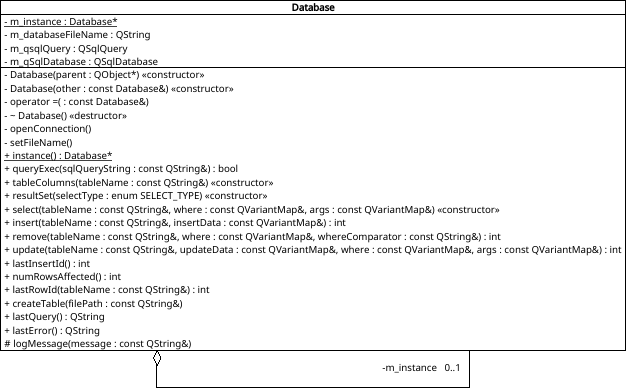
\includegraphics[scale=0.5]{diagrama_de_classe_Database}
	\centering
	\caption{Diagrama da classe Database}
\end{figure}

\subsubsection{O Componente DatabaseComponent}\label{sec:solucao-desenvolvida}
....


\subsection{O Componente UserProfile}\label{sec:solucao-desenvolvida}
....


\subsection{O Componente BasePage}\label{sec:solucao-desenvolvida}
....


\subsection{Componentes Visuais}\label{sec:solucao-desenvolvida}
....


\subsection{Fluxo de execução}\label{sec:solucao-desenvolvida}
....
%Adicionar um diagrama de sequência que mostre a inicialização, carregamento dos plugins e configuração geral do aplicativo%


\subsection{Métodos para utilização da arquitetura}
-- descrever o README do projeto no github

OU:
Exemplo (a ser editado): Para se utilizar a arquitetura desenvolvida, deve-se seguir uma determinada ordem de atividades (Figura 26), que deve se iniciar no nível arquitetural “escopo” (seção 3.1), passando pelos níveis arquiteturais “modelo de negócios” (seção 3.2) e “modelo de sistema” (seção 3.3), até chegar ao nível arquitetural “modelo tecnológico” que deve ser criado pelo usuário desta arquitetura.